\documentclass[11pt]{article}
\usepackage{amssymb, amsmath, libertine, hyperref, xcolor, booktabs, enumitem, microtype}
\usepackage[T1]{fontenc}
\usepackage[margin=1in]{geometry}
\usepackage{tikz}
\newcommand{\gridxy}[4]{% xmin xmax ymin ymax -- gridlines exactly on the ticks
  \foreach \gX in {#1,...,#2} \draw[gray!25] (\gX,#3) -- (\gX,#4);
  \foreach \gY in {#3,...,#4} \draw[gray!25] (#1,\gY) -- (#2,\gY);}
\definecolor{dark-red}{rgb}{0.4,0.15,0.15}
\definecolor{blue-g}{rgb}{0.15,0.28,0.45}
\hypersetup{colorlinks, linkcolor=dark-red, urlcolor=dark-red}
\setlist[enumerate,1]{label=\textbf{(\alph*)}, leftmargin=*, itemsep=7pt, topsep=5pt}
\setlist[enumerate,2]{label=(\roman*), leftmargin=*, itemsep=2pt, topsep=2pt}
\pagestyle{empty}
\newcommand{\prob}[2]{\medskip\noindent\textbf{\large #1}\hfill\textit{#2}\par\smallskip}
\newenvironment{statement}{\par\color{gray!55!black}}{\par\medskip}
\newif\ifgradernotes
\ifdefined\withgradernotes \gradernotestrue \fi
\newcommand{\graders}[1]{\ifgradernotes\par\medskip\noindent
  \fcolorbox{blue-g}{blue-g!6}{\parbox{\dimexpr\textwidth-2\fboxsep-2\fboxrule}{\small
  \textbf{\color{blue-g}For graders.} #1}}\par\fi}
\begin{document}
\begin{center}
{\Large\bfseries Math 111: Calculus \quad Practice Exam 3 --- Solutions}\ifgradernotes\\[3pt]
{\large\color{blue-g} with grading notes --- not for students}\fi
\end{center}

\medskip
\noindent Problem statements are in gray. These are written out in full. On the exam you
would not need this much prose, but you would need the \emph{reasons}, and every reason
here is one that earns marks.

\bigskip\hrule
\prob{1. Rain, from a rate}{}
\begin{statement}
During a storm, the rate at which rain fell, $r(t)$ in millimeters per hour, was
recorded every hour:
\smallskip
\begin{center}
\begin{tabular}{@{}lrrrrr@{}}
\toprule
$t$ (hours) & 0 & 1 & 2 & 3 & 4\\
$r(t)$ (mm/hr) & 0 & 2 & 5 & 9 & 14\\
\bottomrule
\end{tabular}
\end{center}
\smallskip
Assume $r$ is increasing on $[0,4]$.
\end{statement}
\begin{enumerate}
\item {\color{gray!55!black}In a sentence, with units, say what $\int_0^4 r(t)\,dt$ means.}

\smallskip
$\int_0^4r(t)\,dt$ is the total depth of rain, in millimeters, that fell during the
four hours: (mm/hr)$\times$(hr) $=$ mm.
\item {\color{gray!55!black}Compute $L_4$ and $R_4$, with units. Which is an over-estimate and which an
under-estimate of $\int_0^4 r(t)\,dt$? Explain with a picture, not a rule.}

\smallskip
$\Delta t=1$. $L_4=1\cdot(0+2+5+9)=16$ mm and $R_4=1\cdot(2+5+9+14)=30$ mm. Since $r$
is increasing, on each hour the left rectangle uses the smallest rate on that hour and
sits under the graph, so $L_4$ is an under-estimate; the right rectangle uses the largest
and sticks above, so $R_4$ is an over-estimate.
\item {\color{gray!55!black}Compute the trapezoid estimate $T_4$. The differences in the table suggest $r$ is
concave up; assuming it is, is $T_4$ too large or too small? Explain with a picture of a
single subinterval.}

\smallskip
$T_4=\tfrac12(L_4+R_4)=23$ mm. The differences $2,3,4,5$ grow, so the rate rises faster
and faster: concave up. On one subinterval the trapezoid's top edge is the chord joining
the two readings, and for a concave-up graph the chord lies above the curve. So the
trapezoid contains extra area and $T_4$ is too large.
\item {\color{gray!55!black}Use the readings at $t=1$ and $t=3$ to compute the midpoint estimate $M_2$. Assuming
$r$ is concave up, is it too large or too small? Combine your answers to (c) and (d) into
an interval that must contain the true total rainfall.}

\smallskip
$M_2=2\big(r(1)+r(3)\big)=2(2+9)=22$ mm. On one subinterval the midpoint rectangle has
the same area as the trapezoid under the tangent line at the midpoint (the tangent cuts a
triangle off one side and adds an equal one on the other). For a concave-up graph the
tangent line lies below the curve, so $M_2$ is too small. Hence
$22\le\int_0^4r(t)\,dt\le23$ mm.
\end{enumerate}

\newpage
\prob{2. Accumulating a graph}{}
\begin{statement}
The graph of $f$ on $[0,8]$ is below; it is made of straight segments. Let
\[A(x)=\int_0^xf(t)\,dt\qquad\text{for }0\le x\le8.\]
\begin{center}
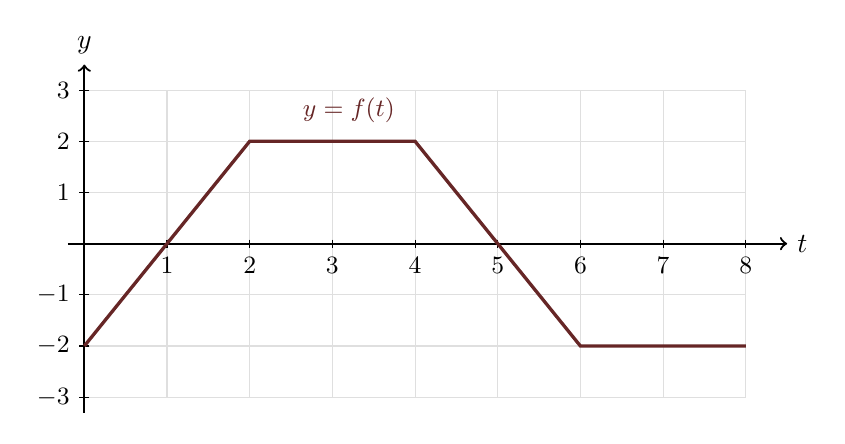
\begin{tikzpicture}[x=1.05cm,y=0.65cm]
  \gridxy{0}{8}{-3}{3}
  \draw[->,thick] (-0.2,0) -- (8.5,0) node[right] {$t$};
  \draw[->,thick] (0,-3.3) -- (0,3.5) node[above] {$y$};
  \foreach \x in {1,...,8} \draw (\x,0.08) -- (\x,-0.08) node[below,font=\small] {\x};
  \foreach \y in {-3,-2,-1,1,2,3} \draw (0.06,\y) -- (-0.06,\y) node[left,font=\small] {$\y$};
  \draw[very thick, dark-red] (0,-2) -- (2,2) -- (4,2) -- (6,-2) -- (8,-2);
  \node[dark-red,font=\small] at (3.2,2.6) {$y=f(t)$};
\end{tikzpicture}
\end{center}
\end{statement}
\begin{enumerate}
\item {\color{gray!55!black}Find $A(1)$, $A(2)$, $A(5)$ and $A(8)$.}

\smallskip
$A(x)$ is the signed area from $0$ to $x$. The segment from $(0,-2)$ to $(2,2)$ crosses
the axis at $t=1$. $A(1)=-\tfrac12\cdot1\cdot2=-1$. $A(2)=-1+1=0$. On $[2,4]$ the area is a
$2\times2$ rectangle, so $A(4)=4$; the segment from $(4,2)$ to $(6,-2)$ crosses at $t=5$, so
$A(5)=4+1=5$. Then $A(6)=5-1=4$ and $A(8)=4-2\cdot2=0$.
\item {\color{gray!55!black}On which intervals is $A$ increasing, and on which decreasing? Find every local maximum
and local minimum of $A$ in $(0,8)$, and the global maximum and minimum of $A$ on $[0,8]$.}

\smallskip
By the Second FTC, $A'=f$. So $A$ increases where $f>0$, on $(1,5)$, and decreases
where $f<0$, on $(0,1)$ and $(5,8)$. $f$ changes from negative to positive at $t=1$: local
minimum $A(1)=-1$. $f$ changes from positive to negative at $t=5$: local maximum $A(5)=5$.
Comparing with the endpoints $A(0)=0$ and $A(8)=0$: the global maximum is $5$ at $x=5$
and the global minimum is $-1$ at $x=1$.
\item {\color{gray!55!black}Find $A'(3)$ and $A'(7)$, and say which theorem you are using. Where is $A$ concave up,
concave down, and straight?}

\smallskip
Second FTC: $A'(x)=f(x)$ because $f$ is continuous. So $A'(3)=f(3)=2$ and $A'(7)=f(7)=-2$.
Concavity of $A$ comes from the slope of $f$ (since $A''=f'$): $A$ is concave up on $(0,2)$
where $f$ increases, a straight line of slope $2$ on $(2,4)$, concave down on $(4,6)$ where
$f$ decreases, and a straight line of slope $-2$ on $(6,8)$.
\item {\color{gray!55!black}A classmate writes: ``$A'(x)=f(x)$, and the largest value of $f$ on $[0,8]$ is $2$,
which $f$ first reaches at $x=2$. So $A$ has its maximum at $x=2$.'' Find the first wrong
step, say why it is wrong, and say where $A$ does have its maximum.}

\smallskip
The first two sentences are true. The wrong step is the conclusion: the largest value of
$f=A'$ is where $A$ is \emph{rising fastest}, not where $A$ is largest. $A$ keeps rising as
long as $f>0$, so it is still increasing at $x=2$ and on through $x=5$. The maximum of $A$
is at $x=5$, where $f$ changes sign from positive to negative, and $A(5)=5$.
\end{enumerate}

\newpage
\prob{3. Evaluating with the FTC}{}
\begin{statement}
Use the Fundamental Theorem of Calculus. Show the antiderivative you use, and check it
by differentiating.
\end{statement}
\begin{enumerate}
\item {\color{gray!55!black}$\displaystyle\int_1^4\Big(3\sqrt x-\frac2{x^2}\Big)\,dx$}

\smallskip
An antiderivative is $F(x)=2x^{3/2}+\frac2x$ (check: $F'(x)=3x^{1/2}-\frac2{x^2}$).
So the integral is $F(4)-F(1)=(16+\tfrac12)-(2+2)=\tfrac{25}2$.
\item {\color{gray!55!black}$\displaystyle\int_0^{\pi/2}\cos x\,dx$, and say in a sentence what this number means
in terms of a graph.}

\smallskip
$\sin x$ is an antiderivative of $\cos x$, so the integral is $\sin\frac\pi2-\sin0=1$.
It is the area of the region under $y=\cos x$ above the $x$-axis from $0$ to $\frac\pi2$
(the region lies above the axis, so signed area is area).
\item {\color{gray!55!black}The average value of $\sin x$ on $[0,\pi]$.}

\smallskip
$\frac1{\pi-0}\int_0^\pi\sin x\,dx=\frac1\pi\big[-\cos x\big]_0^\pi=\frac1\pi(1+1)
=\frac2\pi\approx0.64$.
\item {\color{gray!55!black}A classmate writes: ``An antiderivative of $\frac1x$ is $\ln|x|$, so
$\int_{-1}^{2}\frac1x\,dx=\ln|2|-\ln|-1|=\ln2$.'' Is this right? Find the first wrong
step, and say what hypothesis of the theorem is involved.}

\smallskip
It is not right. The antiderivative is correct ($\frac d{dx}\ln|x|=\frac1x$ for
$x\neq0$). The first wrong step is applying the FTC on $[-1,2]$: the theorem requires $f$
to be continuous on the whole interval, and $\frac1x$ is not even defined at $0$, where it
blows up. The integral does not exist, and $\ln2$ is meaningless here. (The same
antiderivative is fine on $[1,2]$, which stays on one side of $0$.)
\end{enumerate}

\newpage
\prob{4. Differentiating accumulations}{}
\begin{enumerate}
\item {\color{gray!55!black}Find each derivative, and say which rule or theorem you use.
\begin{enumerate}
\item $\displaystyle\frac{d}{dx}\int_2^x\sin(t^2)\,dt$
\item $\displaystyle\frac{d}{dx}\int_x^5\sqrt{1+t^4}\,dt$
\item $\displaystyle\frac{d}{dx}\int_0^{x^3}e^{-t^2}\,dt$
\end{enumerate}}

\smallskip
(i) Second FTC: $\sin(x^2)$. (ii) Flip the limits, $\int_x^5=-\int_5^x$, then Second FTC:
$-\sqrt{1+x^4}$. (iii) This is $H(x^3)$ where $H(u)=\int_0^ue^{-t^2}dt$ has $H'(u)=e^{-u^2}$;
by the chain rule the derivative is $e^{-(x^3)^2}\cdot3x^2=3x^2e^{-x^6}$.
\item {\color{gray!55!black}Let $G(x)=\int_0^x(t^2-3t)\,dt$. Without finding a formula for $G$, find the critical
numbers of $G$ and classify each as a local maximum, local minimum, or neither.}

\smallskip
By the Second FTC, $G'(x)=x^2-3x=x(x-3)$, so the critical numbers are $0$ and $3$. The
sign of $G'$ is $+$ on $(-\infty,0)$, $-$ on $(0,3)$, $+$ on $(3,\infty)$. First derivative
test: local maximum at $x=0$, local minimum at $x=3$.
\item {\color{gray!55!black}Let $A(x)=\int_1^x\sqrt{t^3+1}\,dt$. Find the tangent line to $A$ at $x=1$ and use it to
estimate $A(1.1)$. Is your estimate too large or too small? Explain.}

\smallskip
$A(1)=\int_1^1=0$ and $A'(1)=\sqrt{1^3+1}=\sqrt2$ by the Second FTC. Tangent line:
$L(x)=\sqrt2\,(x-1)$, so $A(1.1)\approx0.1\sqrt2\approx0.141$. Since
$A''(x)=\frac d{dx}\sqrt{x^3+1}=\frac{3x^2}{2\sqrt{x^3+1}}>0$, $A$ is concave up near $1$,
its graph lies above its tangent line, and the estimate is too small. (The true value is
about $0.147$.)
\end{enumerate}

\end{document}
